%!TEX root = paper.tex
%
\begin{algorithm}
\KwData{   $z \in \mathbb{N}_{>0}$; 
            $\mathbf{X}^{(t)}$,$\mathbf{X}^{(t+1)}$,$\dots$, $\mathbf{X}^{(t+z)}$; $\mathbf{U}^{(t)}$,$\mathbf{U}^{(t+1)}$,     
                $\dots$, $\mathbf{U}^{(t+z)}$;
            $\mathbf{T}^{(t)}$,$\mathbf{T}^{(t+1)}$,$\dots$, $\mathbf{T}^{(t+z)}$; 
            We assume that we track a set of defined hashtags so that $N_h^{(t)}  = N_h^{(t+1)} = \dots = N_h^{(t+z)}  $, 
                and in particular that all the rows of $\mathbf{T}$ matrices are equal.
  }
 \KwResult{     
            Two vectors $\textbf{v}_x$,$\textbf{v}_u$ of size $N_h^{(t)}$ containing for each hashtag 
			a stability score over the content matrix $\mathbf{X}$ and       
            user interaction matrix $\mathbf{U}$.
            
 }
 \ForAll{ $i \in {1,2,\dots,N_h}$}{
    $s_x = 0$\;
    $s_u = 0$\;
     \ForAll{ $a \in {t,t+1,\dots,t+z-1}$}{
        $s_x \mathrel{+}= cos( (\mathbf{T}^{(a)} \mathbf{X}^{(a)}){\e}^T_i , (\mathbf{T}^{(a+1)} \mathbf{X}^{(a+1)}){\e}^T_i )$\;
        $s_u \mathrel{+}= cos( (\mathbf{T}^{(a)} \mathbf{U}^{(a)}){\e}^T_i , (\mathbf{T}^{(a+1)} \mathbf{U}^{(a+1)}){\e}^T_i )$\;
     }
     $\textbf{v}_x[i] = \frac{s_x}{z}$\;
     $\textbf{v}_u[i] = \frac{s_u}{z}$\;
 }
\caption{Hashtag stability scores}
 \label{alg:hashtag_stability_scores}
\end{algorithm}
\vspace{-0.4cm}
In order to accurately answer the research questions posed in Section \ref{sec:introduction}, and evaluate
our algorithm we need a dataset where the topics persist over a period of time, 
and also has a social community that accompanies it.   
We use the public dataset which was released in 2013 \cite{YatesTrumper:2013} consisting of all the articles published from 80 international 
news sources such as CNN, BBC, Aljazeera during a period of 14 days. Each news article consists of the textual content
of the article (via \texttt{html}) and a list of all tweets which link to that article over a period 
12 hours from the article's publication. The tweets containing links 
to the news articles were also collected.  From the tweets, two features were extracted: 
the author of the tweet and the hashtags present in the tweet.  The information about the author
of the tweet was used to detect the community information.  The hashtags in the tweets
were used as the groundtruth topic of the document which the tweet linked to \cite{Tsur:2012}.\footnote{We hereby use the words topic and hashtag somewhat interchangeably.}
Most of the articles were associated to a hashtag.  We discarded the ones which did not correspond to any hashtag.  
Since we wish to \emph{track} topics over
a period of time, we consider only those hashtags that appear every day (and thereby pruning 
the number of articles even further). Moreover, to avoid data sparsity of articles, 
we keep only those hashtags that have at least five articles per day. 
After all the filtering, we end up with $33,387$ articles (from an original set of $53,784$)  associated to $384$ different hashtags.
For details about
data acquisition, refer to \cite{YatesTrumper:2013}.
\subsection{Stability of Tags}\label{subsec:hashtag_stability}
\begin{figure}
\begin{center}
    \centering
    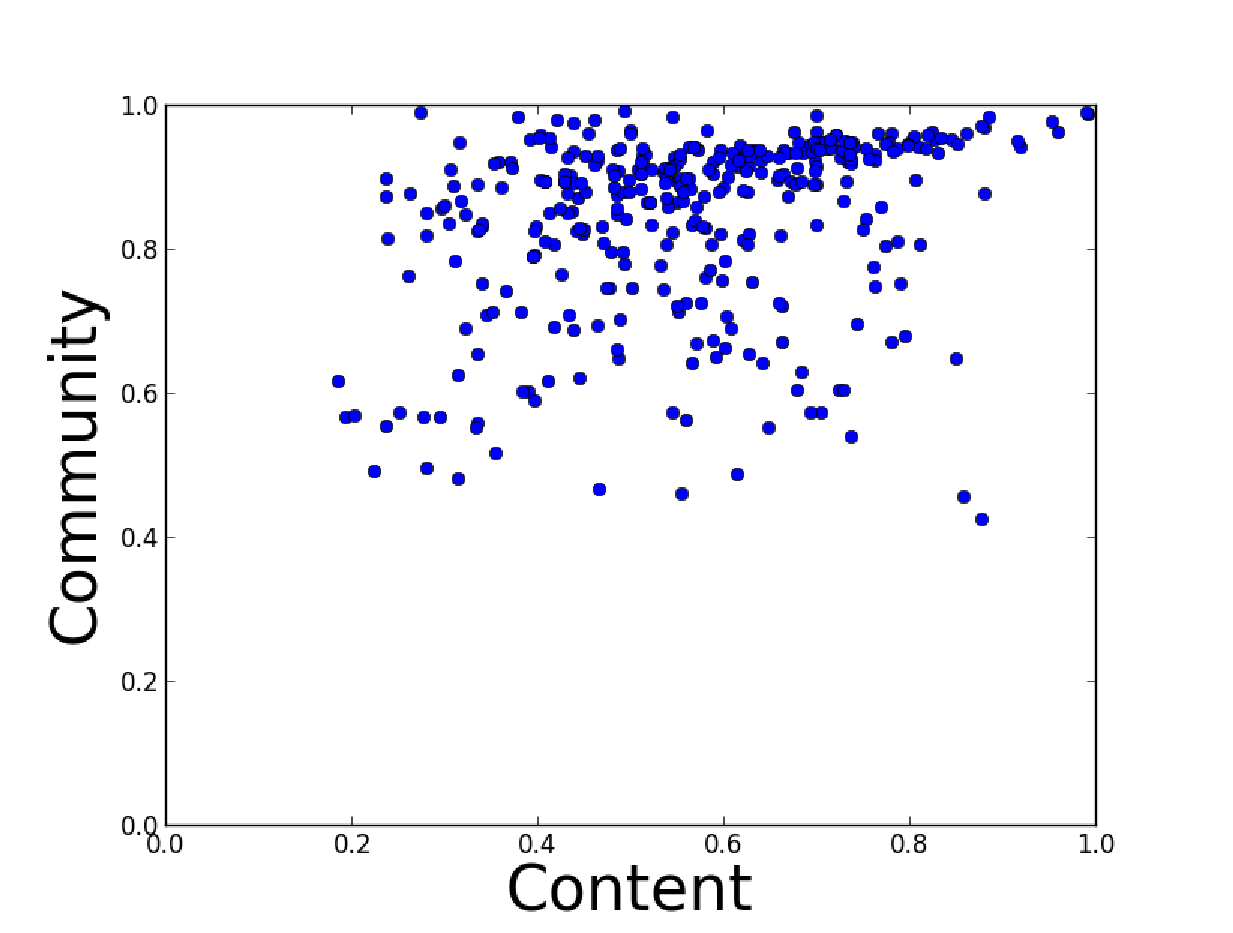
\includegraphics[width=0.5\textwidth]{KDD/images/Text-Vs-Users-sNMF-dots-new}            
\end{center}
  \caption[Stability of hashtags]{{This figure illustrates the stability of hashtags in terms of content and community information.  Each dot in the figure
is a hashtag.  The x-axis and y-axis represent content and community stability.  The content and community stability scores are 
calculated according to Algorithm \ref{alg:hashtag_stability_scores}.}  }
\label{fig:Stability}
\vspace{-0.5cm}
\end{figure}
\begin{table}
\begin{center}
\begin{minipage}[b]{1\linewidth}
{\tiny
\begin{tabular}{|lclclc|}
\multicolumn{6}{c}{\small{Twitter News Dataset}} \cr
\multicolumn{2}{c}{\bf Text-Stable} & \multicolumn{2}{c}{\bf Community-Stable} & \multicolumn{2}{c}{\bf Mixed} \cr
\#birdflu &  & \#facts &  & \#egitto3000 & \cr
\#h7n9 &  & \#celeb &  & \#hindi &  \cr
\#google &  & \#nyt &  & \#tahrir & \cr
\#football &  & \#gossip &  & \#alarabiya &  \cr
\#taxes & & \#followfriday & & \#vrwc &  \cr
\#bangladesh & & \#cbs &  & \#jan25 &  \cr
\#chinese &  & \#businessangel & & \#news &  \cr
\#climatechange &  & \#aje &  & \#rwnjalert &  \cr
\#climate &  & \#fem2 &  & \#bigtweet &  \cr
\#nkorea &  & \#opanews &  & \#business &  \cr
\#immigration &  & \#tf &  & \#india &  \cr
\#iran &  & \#interesting &  & \#smallbusiness & \cr
\#gun &  & \#top & & \#nhl &  \cr
\#lgbt &  & \#cincinnati &  & \#forbes &  \cr
\#dprk &  & \#thn24en & & \#buisnessguide &  \cr
\#nba &  & \#ihatetimwaterman &  & \#tcot &  \cr
\#japan &  & \#stopoccopywaste &  & \#financenews &  \cr
\#tax &  & \#divalishdesigns &  & \#adityaramadana & \cr
\#nuclear & & \#informate &  & \#shubhamconsultants & \cr
\#education & & \#olympic &  & \#money &  \cr
\end{tabular}
} %tiny
\centering 
\end{minipage}
\caption[A list of the top hashtags in each category.]{{This table lists the top-$20$ hashtags found in the content stable, community stable and mixed stable categories.
Basically these are closest $20$ points by Euclidean distance from $(1,0)$, $(0,1)$ and $(1,1)$ in Figure \ref{fig:Stability}
for content stable, community stable, and mixed stable hashtags respectively.  These were used as the groundtruth
for evaluating topic discovery (more details on evaluation in Section \ref{sec:experiments}).}}
\label{tab:tags}
\end{center}
\vspace{-0.8cm}
\end{table}

Recall that we use the hashtags as the groundtruth
topic of the text document.
Keeping in mind our research questions from Section \ref{sec:introduction}, we wanted to detect the three different
categories of hashtags for each dataset.
The first category of hashtags are those that are stable in terms of content, but relatively unstable in terms of community; 
meaning that the content corresponding to these hashtags does not evolve much over the period of interest, but the community
of users who tweet about these hashtags evolves quite a bit.
We call this set \emph{content stable} hashtags.  These are the supposedly `easier' topics where one may expect
that the presence of community may not particularly help in better topic discovery.
The second category of hashtags are those that are stable in terms of their community, but the content evolves a lot;
meaning that the community of users that show an interest on these tags stays relatively unchanged over a period of time,
but the actual content (in terms of vocabulary) changes a lot.
We call this set \emph{community-stable} hashtags.  These are the supposedly more difficult topics where using
the content alone may yield only poor performance, since by definition the content is not very stable.
The third category of hashtags are those that are stable in terms of both content and community, called \emph{mixed-stable}
hashtags.  
Intuitively, we posit that our model would work particularly well in discovering and monitoring those topics which 
have a stable community of active users over the period
of interest, but have a content which is evolving a lot (these are community-stable hashtags).

Following the notation specified in Section \ref{sec:content_and_networks}, we explain how we determine the 
tags which fall into the content-stable, community-stable, and mixed-stable categories.
Let us consider matrix $\mathbf{T}^{(t)}$ of size $N_h^{(t)} \times N_d^{(t)}$, 
where  $N_h^{(t)}$ is the number of hashtags produced at time $t$ and 
$N_d^{(t)}$ is the number of documents arriving at time $t$.
In particular, $\mathbf{T}^{(t)}(i,j) = 1$ if the document $j$ has been mentioned in a tweet
that contains the hashtag $i$, and $0$ otherwise.  Algorithm \ref{alg:hashtag_stability_scores} explains
how we compute a stability score for each hashtag in terms of their content and community. The essence of Algorithm
\ref{alg:hashtag_stability_scores} is as follows: by simply averaging all the documents belonging to a particular
hashtag, we obtain a representation for each hashtag in terms of features extracted from the documents. Following this procedure, each hashtag can consists of a (centroid) vector of  $N_f$ entries (i.e., in a bag-of-words representation).  We compare this representation with a similar
representation obtained for the same hashtag at the next time step using cosine similarity.  We then average
all the similarities obtained across the consecutive time steps for each hashtag.

Refer to Figure \ref{fig:Stability}.  Note that, in such a figure, the point $(1,0)$ represents perfect content stability, and zero community
stability.  To determine the set of hashtags that belong to the \emph{content stable} set, we calculate the Euclidean distance between
$(1,0)$ and all the other hashtags, and rank them in the increasing order of their distances.  Likewise for \emph{community stable} and
\emph{mixed stable} sets (using respectively the Euclidean distances to points $(0,1)$ and $(1,1)$).  
Some examples of content stable hashtags are \texttt{\#football} and \texttt{\#h7n9}; community stable hashtags,
\texttt{\#celeb} and \texttt{\#gossip} and mixed stable hashtags \texttt{\#alarabiya} and \texttt{\#forbes}.
\vspace{-0.2cm}
